
\documentclass{article}
\usepackage[utf8]{inputenc}
\usepackage{mathtext}
\usepackage{amsmath}
\usepackage[colorlinks=true, linkcolor=blue]{hyperref}
\usepackage[T1]{fontenc}
\usepackage[utf8]{inputenc}
\usepackage[english, bulgarian, russian]{babel}
\usepackage{tikz}
\usepackage{pgfplots}
\usepackage{indentfirst}
\usepackage[export]{adjustbox}
\usepackage{lipsum} % sample text
\usepackage{floatflt}
\usepackage{multirow}
\usepackage{geometry} \geometry{verbose,a4paper,tmargin=2cm,bmargin=2cm,lmargin=1.5cm,rmargin=1.5cm}
\setlength{\parindent}{0.65cm}
\setlength{\parskip}{0.15cm}

\usepackage{wrapfig}
\usepackage{array,graphicx,caption}


%Матеша
\usepackage{amsmath,amsfonts,amssymb,amsthm,mathtools} % AMS
\usepackage{icomma} % "Умная" запятая

%\mathtoolsset{showonlyrefs=true} % Показывать номера только у тех формул, на которые есть \eqref{} в тексте.

%% Шрифты
\usepackage{euscript}	 % Шрифт Евклид
\usepackage{mathrsfs} % Красивый матшрифт

%% Свои команды
\DeclareMathOperator{\sgn}{\mathop{sgn}}

%% Перенос знаков в формулах (по Львовскому)
\newcommand*{\hm}[1]{#1\nobreak\discretionary{}
	{\hbox{$\mathsurround=0pt #1$}}{}}
 \begin{document}
\begin{titlepage}
     \begin{center}
     \large Московский физико-технический институт\\
    (национальный исследовательский университет)\\
    \vspace{4cm}
    \Large Лабораторная работа № 5.2.2(2.3) по курсу \\  Квантовая физика\\
    \vspace{4cm}
    \textbf{\Huge <<Изучение спектров атомов водорода и молекулы йода>>}\\
     \end{center}
    \vspace{5cm}
    {\par \raggedleft \large Выполнили:\\ студентки 3 курса
    103 группы\\ Фитэль Алена \\Флоренская Лидия \par}
    \vspace{3cm}
    \begin{center}
        Москва, 02.10.23 г
    \end{center}
\end{titlepage}
\section*{Введение} \label{sec:Intro}



В работе исследуются : 1) сериальные закономерности в оптическом спектре водорода; 2) спектр поглощения паров йода в видимой области




\begin{wrapfigure}{r}{0.3\textwidth}
\begin{center}
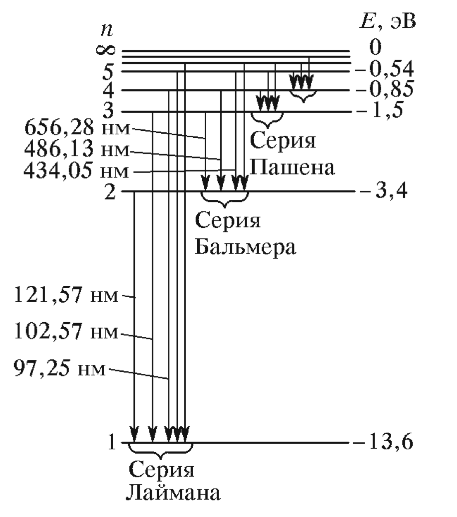
\includegraphics[width=0.3\textwidth]{Screenshot 2023-10-07 at 5.04.51 PM.png}
\caption{Уровни энергии атома водорода и обращование спектральных серий}
\label{vodorod}
\end{center}
\end{wrapfigure}

\subsection*{Спектральные линии водорода}

Атом водорода является простейшей атомной системой; для него уравнение Шредингера может быть решено точно. Поэтому спектр водорода явдяется предметом тщательного экспериментального и теоретического исследования. 

Длины волн спектральных линий водородоподобного атома описываются найденной эмпирически формулой Бальмера
\begin{equation}     
\label{1 formula}
\frac{1}{\lambda_{mn}} = RZ^2 \left(\frac{1}{n^2} - \frac{1}{m^2} \right)~,
\end{equation}

где $R$ - константа, называемая постоянной Ридберга, а $m$ и $n$ - целые числа. 

Эта формула достаточно правильно описывает экспериментальные значения линий водорода при $R = 109 677~см^{-1}$.

Использвание постулатов Нильса Бора с учетом кулоновского взаимодействия между ядром и электроном позволяет легко определить возможные энергетические состояния водородоподобного атома. Если считать ядро неподвижным, то эти энергетичекие состояния определяются выражением
\begin{equation}
    E_n = -\frac{2\pi^2 m_e e^4 Z^2}{h^2} \frac{1}{n^2}
\end{equation}

Это позволяет нам определить возможные частоты излучения атома и объяснить спектральные закономерности (см. \hyperref[vodorod]{Рис. \ref*{vodorod}}). 

Из \hyperref[vodorod]{Рис. \ref*{vodorod}} видно, что линии в спектре водорода можно разложить по сериям. В данной работе изучается серия Бальмера, линии которой лежат в видимой области. Для нее $n = 2$. Величина $m$ для первых четрех линий принимает значение 3,4,5,6. Эти линии обозначаются символами $H_{\alpha}$, $H_{\beta}$, $H_{\gamma}$, $H_{\delta}$.




\begin{wrapfigure}{r}{0.3\textwidth}
\begin{center}
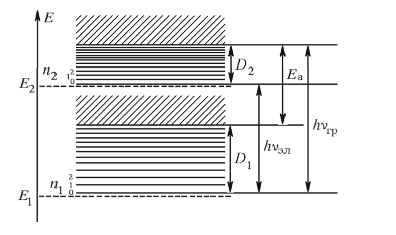
\includegraphics[width=0.3\textwidth]{Screenshot 2023-10-08 at 11.04.01 AM.png}
\caption{Электронные и электронно-колебательные энергетические уровни двухатомной молекулы}
\label{fig:urovni}
\end{center}
\end{wrapfigure}

\subsection*{Оптические переходы в молекулах}
Оптические переходы, связанные с излучением фотонов в видимом диапазоне длин волн, соответствуют переходам между различными электронными состояниями молекулы. 

В спектре излучения просходит наложение колебательного спектра на электронный, и проявляется это в том, что каждой линии электронного перехода соответствует ряд колебательных линий, образующих полосу.



На \hyperref[fig:urovni]{Рис. \ref*{fig:urovni}} схематически показаны энергетические уровни молекулы без учета вращательной структуры. 

Штриховыми линиями показаны чисто электронные уровни $E_1$ и $E_2$, а сплошными - колебательные подуровни этих состояний.Следует подчеркнуть, что минимальное значение колебательной энергии при $n = 0$ отлично от нуля и равно $h\nu/2$. 

Минимальная энергия, которую нужно сообщить молекуле в нижайшем колебательном состоянии $n = 0$, чтобы она диссоциировала, называется энергией диссоциации. Энергии диссоциации молекулы из состояний $n_1 = 0$ и $n_2 = 0$ обозначим через \textsl{Д1} и \textsl{Д2} \hyperref[fig:urovni]{(Рис. \ref*{fig:urovni})}. $E_a$ - энергия возбуждения атома, возникающая при переходе молекула из состояния \textsl{1} в область непрерывного спектра, соответствующего состоянию \textsl{2}. Энергия чисто электронного перехода $E_2 - E_1 = h\nu_{эл}$

В работе мы будем исследовать структуру электронно-колебательного спектра поглощения молекул йода. Все возможные линии поглощения для переходов между колебательными уровнями, налагающимися на два соседних эжлектронных состояния, можно разбить на серии, соответствующие одному и тому же начальному состоянию. Такие серии называются сериями Деландра. 

Энергетическое положение линий поглощения описывается выражением
\begin{equation}
\label{2 formula}
    h \nu_{0,n_2} = (E_2 - E_1)+ h\nu_2 \left( n_2+\frac{1}{2}\right) -\frac{1}{2}h\nu_1
\end{equation}



\begin{wrapfigure}{r}{0.3\textwidth}
\begin{center}
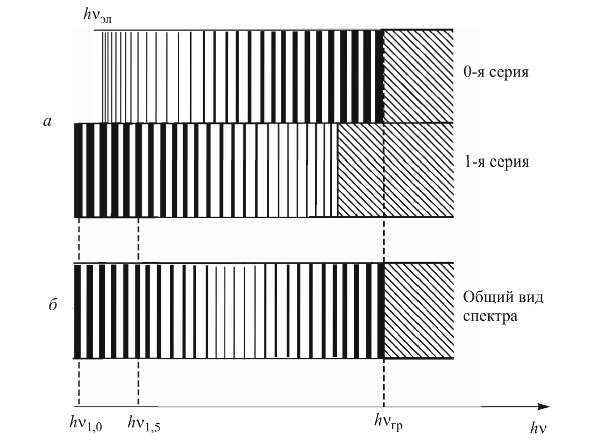
\includegraphics[width=0.3\textwidth]{Screenshot 2023-10-07 at 7.42.22 PM.png}
\caption{Спектр поглощения паров йода}
\label{Yod}
%\vspace{-12mm}
\end{center}
\end{wrapfigure}
\subsection*{Общий вид спектра поглощения йода}
Из рассмотренного ясно, что спектр поглощния паров йода в видимой области при комнатной температуре практически состоит из двух серий Деландра (1-й и 0-й), накладывающихся друг на друга. На \hyperref[Yod]{Рис. \ref*{Yod}а} для наглядности обе серии изображены отдельно. Учтено также распределение интенсивности поглощения между линиями в пределах серии: на рисунке интенсивность условно отражена толщиной линии. Качественно общий вид спетра показан на \hyperref[Yod]{Рис. \ref*{Yod}б}. 




\section{Изучение спектра атома водорода}
Э\,к\,с\,п\,е\,р\,и\,м\,е\,н\,т\,а\,л\,ь\,н\,а\,я  \, у\,с\,т\,а\,н\,о\,в\,к\,а

Для измерения длин волн спектральных линий в работе используется стеклянно-призменный монохроматор-спектрометр УМ-2 \hyperref[UM-2]{(Рис. \ref*{UM-2})}, предназначенный для спектральных исследований в диапазоне от 380 до 1000 нм. 

\begin{wrapfigure}[16]{r}{0.4\textwidth}
\begin{center}
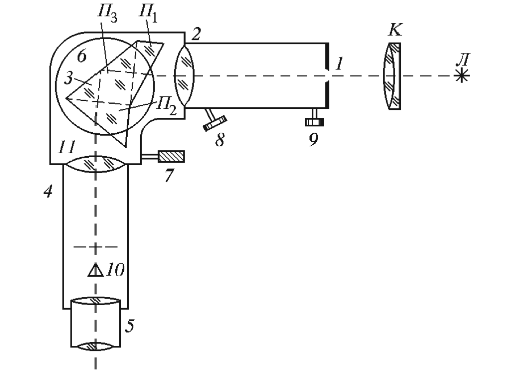
\includegraphics[width=0.4\textwidth]{Screenshot 2023-10-07 at 1.59.20 PM.png}
\caption{Устройство монохроматора УМ-2}
\label{UM-2}
\end{center}
\end{wrapfigure}




В состав прибора УМ-2 входят следующие основные части:
\begin{enumerate}
    \item Входная щель 1, снабженная микрометрическим винтом 9
    \item Коллиаторный объектив 2, снабженный микрометрическим винтом 8, позволяющим смещать объектив относительно щели 1
    \item Сложная спектральная призма 3, состоящая из трех склееных призм \textsl{П1}, \textsl{П2}, \textsl{П3}
    \item Поворотный столик 6б вращающийся вокруг вертикальной оси при помощи микрометрического винта 7 с отсчетным барабаном. На барабан нанесена винтовая дорожка с градусными делениями
    \item Объектив 4 и окуляр 5, составляющие зрительную трубу. Указатель 10 в фокальной плоскости окуляра 5
    \item Массивный корпус 11
    \item Оптическая скамья, по которой могут перемещаться рейтеры с источником света \textsl{Л} и конденсором \textsl{К}.
\end{enumerate}

Спектрометр УМ-2 нуждается в предварительной градуировке. Для градуировки в коротковолновой части спектра удобно применять ртутную лампу ПРК-4, а в длинноволновой и средней части спектра - неоновую лампу. 
%\hyperref[sec:Intro]{to an earlier Section \ref*{sec:Intro}}.

\textbf{Водородная лампа}. В опытах по измерению длин волн бальмеровской серии источником служит водородная трубка Н-образной формы, питаемая от катушки Румкорфа. 

Для увеличения яркости интересующих нас линий атомарного водорода в состав газа, которым заполняют трубку при ее изготовлении, добавляют пары воды. Молекулы воды в электрическом разряде разлагаются, образуя атомарный водород. 

Начинать поиск атомных линий стоит с наиболее интенсивной красной линии $H_{\alpha}$. Вторая линия, $H_{\beta}$ - зелено-голубая. В промежутке между этими линиями распологаются нексолько красно-желтых и зеленых сравнительно слабых молекулярных полос. Третья линия $H_{\gamma}$ - фиолетово-синяя. Четвертая линия, 
$H_{\delta}$ - фиолетовая, и найти ее удается не всегда.


\begin{wrapfigure}{r}{0.4\textwidth} 

  \centering
    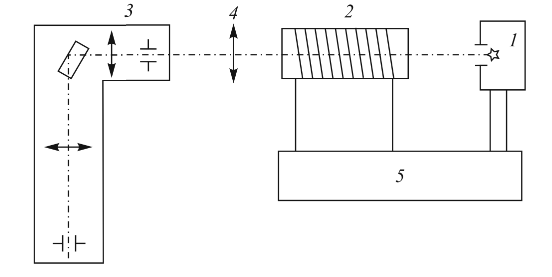
\includegraphics[width=0.4\textwidth]{Screenshot 2023-10-07 at 2.44.47 PM.png}    

  \caption{Схема экспериментальной установки для изучения молекулярного спектра йода}

  \label{UM-2 2}
\end{wrapfigure}

\section{Изучение молекулярного спектра йода}

Молекулярный спектр поглощения паров йода можно наблюдать, используя
\begin{enumerate}
    \item Источник сплошного спектра - лампу накаливания 1, питаемую от блока питания 5
    \item Поглощающую среду - кювету 2 с кристаллами йода, которая подогревается резистором, подключенным вместе с лампой накаливания к блоку питания 5 
    \item Монохраматор УМ-2 3  \hyperref[UM-2]{(Рис. \ref*{UM-2})}
    \item Линзу 4, формирующая пучок света, проходящий через кювету 2 и сфокусированный на входной щели монохроматора 3
\end{enumerate}

В результате подогрева кристаллы йода частично возгоняются, образуя пары с легкой фиолетовой окраской. Монохроматор 3 используется в качестве спектроскопа, позволяющего визуально наблюдать линии поглощения молекул йода на фоне сплошного спектра излучения лампы накаливания в видимой области. 
\newpage
\section{Выполнение задания}
\subsection{Градуировка спектрометра}
Проградуируем спектрометр по спектрам неона и ртути и построим градуировочную кривую, где по оси Х отложены градусные деления барабана, а по оси Y - длины волн соответствующих линий:
\begin{figure}[h!]
    \centering
    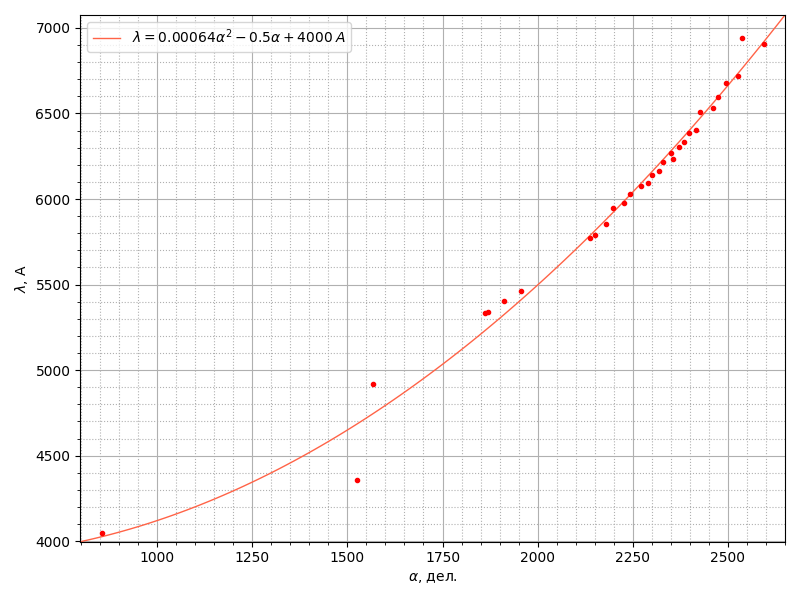
\includegraphics[scale = 0.75]{Figure_1 (1).png}
    \caption{Градуировочная кривая для барабана монохроматора}
    \label{fig:1}
\end{figure}

Коэффициенты в уравнении аппроксимирующей параболы :
\begin{equation*}
    a = (73 \pm 8)\cdot 10^{-5}, ~~~ b = (-53 \pm 29)\cdot 10^{-2}, ~~~c = (40 \pm 2)\cdot 10^2
\end{equation*}

\subsection{Спектр водорода}
Установим на скамью водородную лампу и включим ее в сеть. Измерим положение линий $H_{\alpha}$, $H_{\beta}$, $H_{\gamma}$ и определим с помощью калибровочного графика соотствующие им длины волн, занесем это в  \hyperref[tab:1]{Таблицу \ref*{tab:1}}


\begin{table}[h!]
    \begin{center}
    \begin{tabular}{|c|c|c|c|c|l|l|} \hline  
 & дел, $^o$& $\lambda, \text{\AA}$& $\delta \lambda, \text{\AA}$ &$\lambda_{теор}, \text{\AA}$ & $R,  ~см^{-1}$&$\delta R, ~см^{-1}$\\ \hline  
         $H_{\alpha}$&  2489&  6634&  935 &6563 & 108 531,8&15 296,5\\ \hline  
         $H_\beta$&  1474&  4614&  545 &4861 & 115 590,2&13 653,4\\ \hline  
         $H_{\gamma}$&  821&  4008&  369 &4341 & 118 810,0&10 938,3\\ \hline 
    \end{tabular}
    \caption{Положение линий $H_{\alpha}$, $H_{\beta}$, $H_{\gamma}$}
    \label{tab:1}
    \end{center}
\end{table}
\newpage
\begin{figure}[h!]
    \centering
    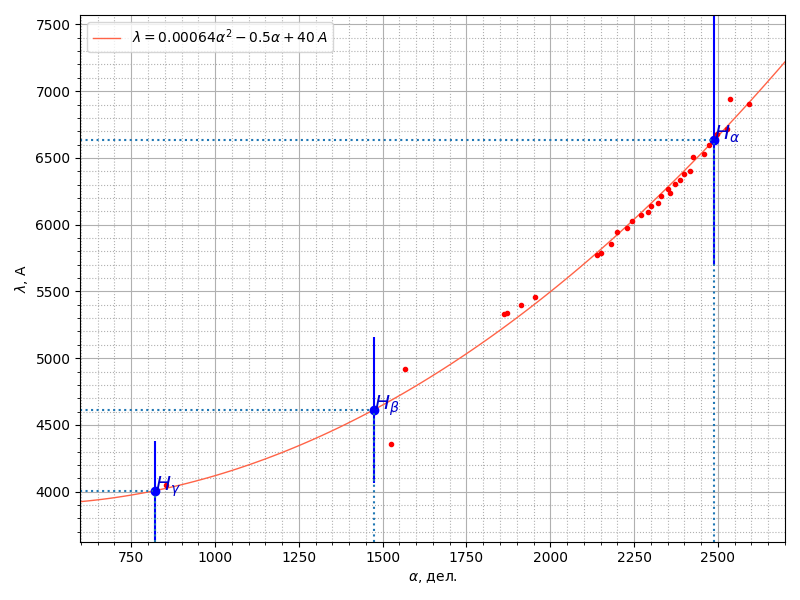
\includegraphics[scale = 0.75]{Figure_2.png}
    \caption{Положение линий $H_{\alpha}$, $H_{\beta}$, $H_{\gamma}$}
    \label{fig:Halpha}
\end{figure}

Проверим, что отношение длин волн водородных линий соответствуют \hyperref[1 formula]{Формуле (\ref*{1 formula})} сериальной закономерности  и для каждой из линий вычислим значение постоянной Ридберга, занесем результаты в  \hyperref[tab:1]{Таблицу \ref*{tab:1}}.

Из  \hyperref[1 formula]{Формулы (\ref*{1 formula})} следует, что 
\begin{equation*}     
\label{}
0.69 = \frac{\lambda_{\beta}}{\lambda_{\alpha}} =  \frac{\left(\frac{1}{2^2} - \frac{1}{3^2} \right)}{\left(\frac{1}{2^2} - \frac{1}{4^2} \right)} = 0.74
\end{equation*}
\begin{equation*}     
\label{}
0.56 = \frac{\lambda_{\gamma}}{\lambda_{\beta}} =  \frac{\left(\frac{1}{2^2} - \frac{1}{4^2} \right)}{\left(\frac{1}{2^2} - \frac{1}{5^2} \right)} = 0.89
\end{equation*}

 Среднее значение вычисленной постоянной Ридберга :
 \begin{equation}
 \label{R}
     R = (114~310,7 \pm 23~238,9)~ см^{-1}
 \end{equation}

Эмперическое же значение:
  \begin{equation*}
     R = 109 ~677,6~ см^{-1}
 \end{equation*}
\newpage

\subsection{Спектр йода}
Установим на скамью кювету с йодом и лампу накаливания. Качественно сопоставим наблюдаемый спектр со спектром поглощения, изображенным на \hyperref[Yod]{Рис. \ref*{Yod}}

Определим и запишем в  \hyperref[tab:2]{Таблицу \ref*{tab:2}} деления барабана монохроматора n, соответствующие:
\begin{enumerate}
    \item линии $h \nu_{1,0}$ - одной из самых длинноволновых хорошо видимых линий поглощение $(n_{1,0})$
    \item линии $h \nu_{1,5}$ - шестой по счету от выбранной длинноволновой линии  $(n_{1,5})$
    \item $h \nu_{гр}$ - границе схождения спектра, т.е. началу сплошного спектра $(n_{гр})$
\end{enumerate}

Проделаем это дважды для понимания точности измерения...

По градуировочной кривой монохроматора определим длины волн линий поглощения йода, соответствующие делениям барабана монохроматора $n_{1,0}$, $n_{1,5}$, $n_{гр}$, запишем результаты в \hyperref[tab:2]{Таблицу \ref*{tab:2}}

\begin{figure}[h!]
    \centering
    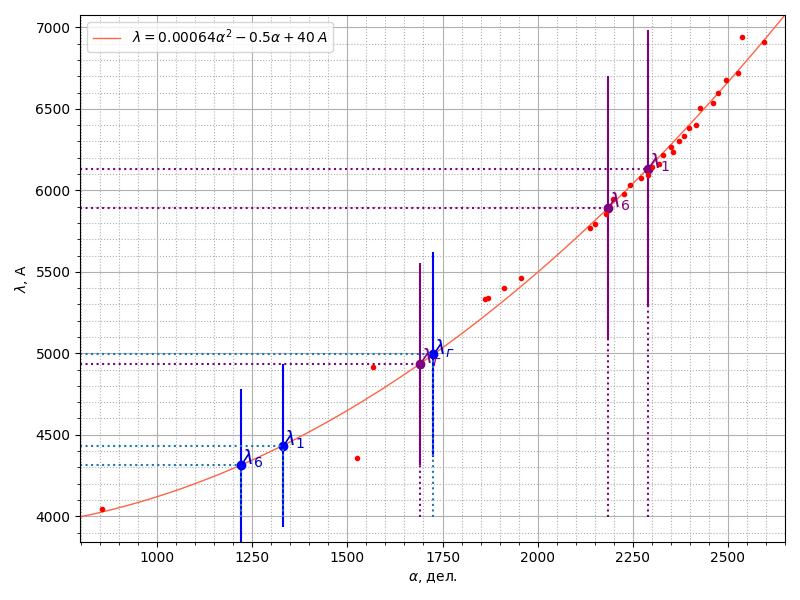
\includegraphics[scale = 0.75]{Figure_3.png}
     \caption{Положение линий $n_{1,0}$, $n_{1,5}$, $n_{гр}$}
    \label{fig:n0,5}
\end{figure}
\begin{table}[h!]
    \begin{center}
        
    
    \begin{tabular}{|c|c|c|c|c|c|} \hline 
 \multicolumn{6}{|c|}{1 измерение}\\ \hline 
         &  дел, $^o$&  $\lambda, \text{\AA}$&  $\delta \lambda, \text{\AA}$  & $\nu, 10^{15}\cdot c^{-1}$& $\delta\nu, 10^{15}\cdot c^{-1}$\\ \hline 
         $n_{1,0}$&  1330&  4400&  502 & 0,68& 0,08\\ \hline 
         $n_{1,5}$&  1220&  4314&  470 & 0,70& 0,08\\ \hline 
          $n_{гр}$&  1726&  4993&  631 & 0,60& 0,08\\ \hline 
         \multicolumn{6}{|c|}{2 измерение}\\ \hline 
         &  дел, $^o$&  $\lambda, \text{\AA}$&  $\delta \lambda, \text{\AA}$  & $\nu, 10^{15}\cdot c^{-1}$& $\delta\nu, 10^{15}\cdot c^{-1}$\\ \hline 
         $n_{1,0}$&  2289&  6132&  849 & 0,49& 0,06\\ \hline 
         $n_{1,5}$&  2186&  5894&  806 & 0,51& 0,06\\ \hline 
          $n_{гр}$&  1690&  4934&  618 & 0,60& 0,08\\ \hline
    \end{tabular}
    \caption{Положение линий $n_{1,0}$, $n_{1,5}$, $n_{гр}$}
    \label{tab:2}
    \end{center}
\end{table}

Вычислим энергию колебательного кванта возбужденного состояния молекулы йода:
\begin{equation}
\label{hnu2}
    h \nu_{2} = \frac{h \nu_{1,5} - h \nu_{1,0}}{5} = 4,3 \cdot 10^{-15} \cdot \frac{(0,70 - 0,68)\cdot 10^{15}}{5} = (0,097 \pm 0,13)~эВ
\end{equation}

Используя полученные в работе результаты, а также данные о том, что энергия колебательного кванта основного состояния $h \nu_{1} = 0,027~эВ$, а энергия возбуждения атома $Е_а = 0,94~эВ$, вычислим:
\begin{enumerate}
    \item Энергию электронного перехода 
    \begin{equation*}
        h \nu_{эл} = E_2 - E_1 \stackrel{\hyperref[2 formula]{Формула (\ref*{2 formula})}}{=} h \nu_{0,n_2} -\left(n_2 + \frac{1}{2} \right)h\nu_2  + \frac{1}{2}h\nu_1 = h \nu_{1,n_2} -\left(n_2 + \frac{1}{2} \right)h\nu_2  + \frac{3}{2}h\nu_1 =
    \end{equation*}
    \begin{equation*}
        = h \nu_{1,0} -\left(\frac{1}{2}\right)h\nu_2  + \frac{3}{2}h\nu_1 = (2,3 \pm 0,4) ~эВ 
    \end{equation*}
    \item  Энергию диссоциации молекулы в основном состоянии \textsl{Д1}
    \begin{equation}
    \label{d1}
        \textsl{Д1} \stackrel{\hyperref[fig:urovni]{Рис. \ref*{fig:urovni}}}{=} h \nu_{гр}  - Е_а = 1,64 \pm 0,34~эВ
    \end{equation}
    \item  Энергию диссоциации молекулы в возбужденном состоянии \textsl{Д2}
    \begin{equation}
    \label{d2}
        \textsl{Д2} \stackrel{\hyperref[fig:urovni]{Рис. \ref*{fig:urovni}}}{=} h \nu_{гр}  - h\nu_{эл} = 0,28 \pm  0,41~эВ
    \end{equation}
\end{enumerate}
\section{Итоги}
В данной работе мы 
\begin{enumerate}
    \item Прокалибровали барабан спектрометра по спектрам неона и ртути (см. \hyperref[fig:1]{Рис. \ref*{fig:1}})
    \item Определили координаты линий бальмеровской серии атомарного водорода (см. \hyperref[fig:Halpha]{Рис. \ref*{fig:Halpha}} и  \hyperref[tab:1]{Таблицу \ref*{tab:1}}) и по результатам измерений определили постоянную Ридберга \hyperref[R]{$R$ (\ref*{R})}
    \item Определили координаты нескольких линий молекулярного спектра йода (см. \hyperref[fig:n0,5]{Рис. \ref*{fig:n0,5}} и \hyperref[tab:2]{Таблицу \ref*{tab:2}}); по результатам вычислили энергию колебательного кванта молекулы йода и энергию ее диссоциации в основном и возбужденном состояниях \hyperref[hnu2]{$h \nu_{2}$ (\ref*{hnu2})}, \hyperref[d1]{\textsl{Д1} (\ref*{d1})}, \hyperref[d2]{\textsl{Д2} (\ref*{d2})}
\end{enumerate}
\end{document}   
